\documentclass[fleqn,11pt]{article}

\usepackage{datetime}
\newcommand{\ver}{version 0.10\xspace}
\newdateformat{mydate}{\THEDAY~\monthname[\THEMONTH]~\THEYEAR}
\newcommand{\auth}{Fernando D. Bianchi}
\newcommand{\email}{febianchi@itba.edu.ar}
\newcommand{\web}{http://fdbianchi.github.io}

\usepackage{graphicx,epstopdf}
\usepackage{wrapfig}
%
% margenes
\usepackage[a4paper,left=2.5cm,right=2.5cm,top=2.5cm,bottom=2.5cm]{geometry}
\setlength{\parskip}{2ex}

% fonts
%\usepackage{kpfonts}
%\usepackage{times}
\usepackage{bera}
%\usepackage{lucidabr}
%\usepackage{cmbright}
%\usepackage{inconsolata}
\usepackage[T1]{fontenc}
%
% for link and crossreferences
\usepackage{color} % colores de los hipervículos
\definecolor{clink}{rgb}{0,0,0.4}
\definecolor{ccite}{rgb}{0,0,0.4}
\usepackage[english]{hyperref}   % hipervículos
\hypersetup{colorlinks, backref, pdfpagemode=None, linkcolor=clink,
            citecolor=ccite, urlcolor=clink, pdfhighlight=/I, pdfstartview=FitH,
            pdfauthor=F.D.Bianchi, breaklinks}
\usepackage{url}
\newcommand{\weblink}[1]{\url{#1}}
%
% titles
\usepackage[nobottomtitles*]{titlesec}
\definecolor{MyDarkBlue}{rgb}{0,0.08,0.45}
\titleformat{\chapter}
    {\sffamily\bfseries\LARGE}{}{0ex}{}
\titlespacing*{\chapter}%
    {-0.5cm}{7.5ex plus 0.2ex minus 0.2ex}{3.5ex plus 0.2ex minus 0.2ex}%
\titleformat{\section}%
    {{\color{MyDarkBlue}{\titlerule[1pt]}}%
     \vspace{-0.5ex}%
     \sffamily\bfseries\Large}{\thesection}{1.0em}{}[]%
\titlespacing*{\section}%
    {-0.5cm}{6.5ex plus 0.2ex minus 0.2ex}{3.0ex plus 0.2ex minus 0.2ex}%
\titleformat{\subsection}%
    {\sffamily\bfseries\large}{\thesubsection}{0.8em}{}[]%
\titlespacing*{\subsection}%
    {-0.5cm}{4.5ex plus 0.2ex minus 0.2ex}{2.0ex plus 0.2ex minus 0.2ex}%
\titleformat{\subsubsection}%
    {\sffamily\bfseries\normalsize}{}{0.0em}{}%[\titlerule]%
\titlespacing*{\subsubsection}%
    {0cm}{0.5ex plus 0.1ex minus 0.1ex}{0.1ex plus 0.1ex minus 0.1ex}%
\renewcommand{\abstractname}{\vspace{-\baselineskip}}

% headers
\usepackage{fancyhdr}
\fancypagestyle{headings}{%
    \fancyhf{} % clear all six fields
    \fancyfoot[L]{\small\textcolor{gray}{\lpvtool, \ver~-~\mydate\today}}
    \fancyfoot[R]{\small\textcolor{gray}{\thepage}}
    \renewcommand{\headrulewidth}{0pt}
    \let\FootRule\footrule
    \renewcommand\footrule{\color{gray}\FootRule}    \renewcommand{\footrulewidth}{1pt}}
\pagestyle{headings}

% new environments
\usepackage{enumitem}
\setlist[itemize]{label=-,topsep=0ex,parsep=0ex,partopsep=0ex,%
        leftmargin=3ex,itemsep=1.2ex}

% tables
\usepackage{booktabs,array}
%
% for matlab code
\usepackage{listings}
\usepackage{matlab-prettifier}
\lstdefinestyle{mystyle}{
    style=Matlab-editor,
    basicstyle=\mlttfamily,
    backgroundcolor=\color{gray!15},
    rulecolor=\color{gray!15},
    frame=single,
    xleftmargin=2mm,
    framexleftmargin=1mm,
    framextopmargin=0mm,
    framexbottommargin=0mm,
    aboveskip={1ex},
    belowskip={0.5ex}
}
\definecolor{ccode}{rgb}{0,0.08,0.45}
\lstMakeShortInline[style=mystyle,basicstyle=\mlttfamily\color{ccode}]!
\lstnewenvironment{code}{\lstset{style=mystyle}}{}
\newcommand{\lcode}[1]{\textbf{%
    \lstinline[style=mystyle]{#1}}}

\usepackage{amsmath}
\usepackage{cleveref}
\crefname{figure}{Figure}{Figures}
\crefname{table}{Table}{Tables}
\crefname{section}{Section}{Sections}
\crefname{equation}{}{}
\crefrangeformat{equation}{(#3#1#4)-(#5#2#6)}
\usepackage[numbers]{natbib}

% New commands
\usepackage{amssymb}
\usepackage{mathrsfs,bm}
\newcommand{\p}{\rho}
\newcommand{\Cset}{\mathbb{C}}
\newcommand{\Rset}{\mathbb{R}}
\newcommand{\Pset}{\mathcal{P}}
\newcommand{\Pdset}{\mathcal{P}_d}
\newcommand{\Xu}{\mathbf{X}}
\newcommand{\Yu}{\mathbf{Y}}
\newcommand{\Pu}{\mathbf{P}}
\newcommand{\Su}{\mathbf{S}}
\newcommand{\Tu}{\mathbf{T}}
\newcommand{\Gu}{\mathbf{G}}
\newcommand{\Hu}{\mathbf{H}}
\newcommand{\Qu}{\mathbf{Q}}
\newcommand{\Zu}{\mathbf{Z}}
\newcommand{\Ru}{\mathbf{R}}
\newcommand{\Mu}{\mathbf{M}}
\newcommand{\Au}{\mathbf{\hat A}}
\newcommand{\Bu}{\mathbf{\hat B}}
\newcommand{\Cu}{\mathbf{\hat C}}
\newcommand{\Du}{\mathbf{\hat D}}

\usepackage{accents}
\newcommand{\maxS}[1]{\bar{#1}}
\newcommand{\minS}[1]{\underaccent{\bar}{#1}}
\usepackage{xspace}
\newcommand{\lpvtool}{\textbf{LPVtools}\xspace}
\newcommand{\ie}{{\em i.e.}\xspace}
\newcommand{\eg}{{\em e.g.}\xspace}
\newcommand{\etal}{{\em et al.}\xspace}
\newcommand{\example}{\noindent\emph{Example:}\xspace}

\newcommand{\td}{\textcolor{red}{\textbf{~$\blacktriangleright$~ToDo~$\blacktriangleleft$~}}}
\newcommand{\ck}{\textcolor{green}{\textbf{~$\blacktriangleright$~Check~$\blacktriangleleft$~}}}

\usepackage[toc]{multitoc}
\renewcommand*{\multicolumntoc}{2}
\setlength{\columnseprule}{0.5pt}

\sloppy

\begin{document}

\title{\lpvtool: a toolbox to design gain-scheduled LPV controllers.}
\author{\auth\\\weblink{\web}~-~\email}
\date{\mydate\today}
%\date{\ver~-~\mydate\today}
%
\maketitle{}

\begin{abstract}
    \lpvtool is a small toolbox aimed to design gain-scheduled Linear Parameter Varying (LPV) controllers. It provides tools for modelling, setting specifications, synthesizing controllers and evaluating results. This report presents a brief introduction to the use of objects and functions available in the toolbox.
\end{abstract}

%\renewcommand{\baselinestretch}{0.75}\normalsize
%\tableofcontents
%\renewcommand{\baselinestretch}{1.0}\normalsize


\section{Getting started}\label{sec:gt}

\lpvtool implements several synthesis procedures for linear parameter varying (LPV) systems. The toolbox provides a set of objects for modelling and analyzing LPV systems and the function !lpvsyn! for designing gain-scheduled LPV controllers. The basic use is shown in the following code:

\begin{code}
% definition of the parameter set
pv = pset.Box([0 1;0 2]);
% definition of the LPV model (affine in this case)
A(:,:,1) = [-2 1; -1 -2];
A(:,:,2) = [-1.3 0.1; -0.1 -1.3];
A(:,:,3) = [-0.5 0; 0 -0.5];
B        = [1;1];
C(:,:,1) = [10 10];
C(:,:,2) = [2 2];
C(:,:,3) = [5 5];
D = zeros(1,1);
pdG = pass(A,B,C,D,pv);
pdG.u = 'u';    pdG.y = 'y';
% definition of the augmented plant
sb    = sumblk('e = r - y');
pdGau = connect(pdG,sb,{'r','u'},{'e','u','e'});
% weights
We = tf([0.2 20],[1 1]);
Wu = tf([0.04 0.1],[0.004 1]);
Wout = append(W1,W2,1);
% augmented plant + weights
Gaw = wout*Gau;
% constraints
const(1) = synConst.Gain(1,1:2);
const(2) = synConst.Poles('MaxFreq',1000);
% synthesis
pdK = lpvsyn(pdGaw,3,2,const1);
\end{code}

In the folder !demos!, it can be found several examples showing the use of the toolbox in more complex applications.

\section{Modelling}\label{sec:model}

An LPV model is described by the parameter-dependent system matrices and a set in which the parameters takes values. The following paragraphs present the modelling tools provided by \lpvtool.

\subsection{Parameter sets}\label{ssec:parset}

\lpvtool implements four types of sets in order to state the range of  values that each parameter can take. The description also allows specifying \emph{the rate of variation of each parameter, which always must be in an hypercube}. Notice that the parameters are assumed defined as a column vector, such as:
\begin{equation*}
    \p = \begin{bmatrix}
          \p_1 \\
          \p_2 \\
          \vdots \\
          \p_{n_p}
        \end{bmatrix}.
\end{equation*}

\subsubsection{Box (\texorpdfstring{\lcode{pset.Box}}{pset.Box})}\label{sssec:box}

\begin{wrapfigure}[9]{r}{6cm}
  \vspace{-5ex}
  \centering
  \includegraphics{figs/fig_set_Box.pdf}
\end{wrapfigure}
A box set is an hypercube defined by the range of allowable values for each parameter, \ie,
\begin{equation*}
    \Pset = \left\{\,\p\in\Rset^{n_p}\,:\,\minS{\p}_i\leq\p_i\leq\maxS{\p}_i,\quad i=1,\dots,n_p\,\right\}
\end{equation*}
This kind of set is defined with an object \lcode{pset.Box}.

\example The set
\begin{equation*}
    \Pset = \left\{\,\p\in\Rset^{2}\,:
    \,1\leq\p_1\leq 3,\,-2\leq\p_2\leq 2,
    \,-1\leq\dot\p_1\leq 1,\,-1\leq\dot\p_2\leq 1
    \,\right\}
\end{equation*}
can be defined by any of the three code lines:
\begin{code}
s1 = pset.Box([1 3;-2 2],[-1 1;-1 1]);
s2 = pset.Box([1 3;-2 2],[-1 1]);
s3 = pset.Box([1 3;-2 2],[-1 1],{'rho1','rho2'});
\end{code}

\subsubsection{Grid (\texorpdfstring{\lcode{pset.Grid}}{pset.Grid})}\label{sssec:grid}

\begin{wrapfigure}[9]{r}{6cm}
  \vspace{-5ex}
  \centering
  \includegraphics{figs/fig_set_Grid.pdf}
\end{wrapfigure}
A grid set consists of a grid of points bounded by the hypercube corresponding to the range of allowable values for each parameter, \ie,
\begin{equation*}
    \Pset = \Pset_1 \times \Pset_2 \times \dots \times \Pset_{n_p}
\end{equation*}
where
\begin{equation*}
    \Pset_i = \left\{\minS{\p}_i=\p_{i1}<\p_{i2}<\dots<\p_{i,n_i}=\maxS{\p}_i\right\},
    \quad i=1,\dots,n_p.
\end{equation*}
This kind of set is described with an object \lcode{pset.Grid}.

\example For the set
\begin{equation*}
    \Pset = \{1,1.5,2.0,2.5\}\times\{-1,0,1\},
\end{equation*}
with $-2\leq\dot\p_1\leq 2$ and $\,-2\leq\dot\p_2\leq 2$, two of the following syntaxis can be used:
\begin{code}
subsets = {1:0.5:2.5,-1:0:1};
s1 = pset.Grid(subsets,[-2 2],{'rho1','rho2'});
s2 = pset.Grid([1 2.5;-1 1],[4, 3],[-2 2],{'rho1','rho2'});
\end{code}
In the first syntaxis, the set is defined by one vector for each parameter. In the second, the subsets are automatically computed from the ranges of values and the number of points for each one. In this example, the result is the same set. The first syntaxis is useful to define not equally spaced grids of points.

\subsubsection{Polytope or convex hull (\texorpdfstring{\lcode{pset.Hull}}{pset.Hull})}\label{sssec:hull}

\begin{wrapfigure}[9]{r}{6cm}
  \vspace{-5ex}
  \centering
  \includegraphics{figs/fig_set_Pol.pdf}
\end{wrapfigure}

This kind of sets corresponds to the convex hull of a set of points or vertices $\hat{\p}^i\in\Rset^{n_p}$, \ie,
\begin{equation*}
    \Pset = \mathrm{Co}\left\{\hat{\p}^1,\hat{\p}^2,\dots,\hat{\p}^{n_v}\right\}
\end{equation*}
The object \lcode{pset.Hull} is used to define these sets.

\example The set
\begin{equation*}
    \Pset = \mathrm{Co}\left\{(1,1),(3,3),(4,0.5)(2,3)\right\}
\end{equation*}
can be stated with:
\begin{code}
points = [1 3 4 2;1 3 0.5 3];
s1 = pset.Hull(points,[],{'rho1','rho2'});
\end{code}
Notice that no matter the number of points entered in the set definition, the function automatically finds the convex hull and discard the points inside the hull. Each column of !points! corresponds to one point in the set definition.

\subsubsection{General (\texorpdfstring{\lcode{pset.Gral}}{pset.Gral})}\label{sssec:gral}

\begin{wrapfigure}[9]{r}{6cm}
  \vspace{-5ex}
  \centering
  \includegraphics{figs/fig_set_Gral.pdf}
\end{wrapfigure}

The most general set is defined by a set of points $\p^i\in\Rset^{n_p}$,\ie,
\begin{equation*}
    \Pset = \left\{\p^1,\p^2,\dots,\p^{n_v}\right\}
\end{equation*}
inside a convex hull defined by the $n_v$ vertices $\hat{\p}^i\in\Rset^{n_p}$, \ie,
\begin{equation*}
    \Pset = \mathrm{Co}\left\{\hat{\p}^1,\hat{\p}^2,\dots,\hat{\p}^{n_v}\right\}
\end{equation*}
The object \lcode{pset.Gral} is used to describe this kind of sets. Unlike the set type hull, all points in the set definition are stored in the object.

\example The set
\begin{equation*}
    \Pset = \left\{(1,1),(3,3),(4,0.5)(2,3)\right\}
\end{equation*}
can be described with:
\begin{code}
points = [1 3 4 2;1 3 0.5 3];
s1 = pset.Gral(points,[],{'rho1','rho2'});
\end{code}

\subsubsection{Common functions}\label{sssec:setCommon}

The four set objects have the following functions:
\begin{itemize}
  \item \lcode{plot} provides an illustrative representation in case of sets with $1$, $2$ or $3$ parameters.

  \item \lcode{checkval} checks if a given point is in the set:
\begin{code}
s1 = pset.Box([1 3;-2 2]);
p  = [1.5;1];
checkval(s1,p);
\end{code}

  \item \lcode{cvxdec} produces a convex decomposition, \ie,
        \begin{align*}
            \p &= \sum_{i=1}^{n}\alpha_i\p^{j},
            \quad\alpha_1+\dots+\alpha_n=1,
            \quad \alpha_i\geq0, \;i=1,\dots,n.
        \end{align*}
        In case of box or grid sets, the decomposition is based on the four closest points in the set definition (\eg, $n=4$, in case of two-parameter sets). Otherwise, the decomposition is computed by triangulation with respect to the three closest points in the definition (\eg, $n=3$ in case of two-parameter sets). That is,
\begin{lstlisting}[style=mystyle]
subsets = {[1 2 3],[1 4 6]};
s1 = pset.Grid(subsets);
p  = [1.5;2];
[alpha,idx] = cvxdec(s1,p);
\end{lstlisting}
will return
\begin{lstlisting}[style=mystyle]
alpha = [0.3333 0.3333 0.1667 0.1667]';
idx = [1 2 4 5]
\end{lstlisting}
the point !p! is obtained from
\begin{lstlisting}[style=mystyle]
p = pset.Grid.points(:,idx)*alpha;
\end{lstlisting}

\item \lcode{size} provides the number of parameters and the number of points in the set definition.

\item \lcode{isequal} checks if two sets are equal, \ie, if they have the same parameter rate limits, the same points and the same parameter names.

\item Subsets can be obtained using subscripts. Given a set !s1! with $3$ parameters:
\begin{code}
s2 = s2([1 3]);
\end{code}
    produces a subset with the first and third parameters.

\item \lcode{pvec} can be used to convert the set into !pvec! objects from Lmitools.
\end{itemize}

\subsection{System description}\label{ssec:sysLPV}

An LPV model is described mathematically in the form
\begin{equation*}
    \begin{aligned}
        \dot x &= A(\p)x+B(\p)u,\\
        y &= C(ºp)x+D(\p)u
    \end{aligned}
\end{equation*}
with the parameter $\p\in\Pset$. Three type of models are covered by \lpvtool.

\subsubsection{Affine models}\label{sssec:sysPass}

The system matrices of an affine LPV model of $n_p$ parameters are described as
\begin{equation}\label{eq:affLPVmodel}
    \begin{bmatrix}
        A(\p) & B(\p) \\
        C(\p) & D(\p)
    \end{bmatrix} =
    \begin{bmatrix}
        A_0 & B_0 \\
        C_0 & D_0
    \end{bmatrix} + \sum_{i=1}^{n_p}\p_i
    \begin{bmatrix}
        A_i & B_i \\
        C_i & D_i
    \end{bmatrix},
\end{equation}
where $A_i$, $B_i$, $C_i$ and $D_i$ ($i=0,\dots,n_p$) are constant matrices. The parameters $\p_i$'s take values in a set $\Pset\subset\Rset^{n_p}$ of the form previously described.

\lpvtool includes the object \lcode{pass} to describe affine LPV models. For example, consider the LPV model
\begin{align*}
    \dot{x} &= A(\p)x+Bu,\\
    y &= Cx,
\end{align*}
with
\begin{align*}
    A(\p) &= \begin{bmatrix}
                -3 & 0 \\
                 0 & -6
            \end{bmatrix} + \p
            \begin{bmatrix}
                0.5 & 0.5 \\
               -0.5 & 0.5
            \end{bmatrix},&
    B &= \begin{bmatrix}
          1 \\ 1
        \end{bmatrix},&
    C &= \begin{bmatrix}
          2 & 3
        \end{bmatrix},
\end{align*}
and a parameter set $\Pset = \{\p\in\Rset\,:\,0\leq\p\leq 1\}$. This model is defined as
\begin{code}
A(:,:,1) = [-3 0;0 -6];
A(:,:,2) = [0.5 0.5;-0.5 0.5];
B(:,:,1) = [1;1];
B(:,:,2) = [0;0];
C(:,:,1) = [2 3];
C(:,:,2) = [0;0];
D        = 0;
Pset = pset.Box([2 3])
pdG = pass(A,B,C,D,Pset);
\end{code}
When some of the matrices are constant, a shorter syntaxis can also be used:
\begin{code}
A(:,:,1) = [-3 0;0 -6];
A(:,:,2) = [0.5 0.5;-0.5 0.5];
B        = [1;1];
C        = [2 3];
D        = 0;
Pset = pset.Box([2 3])
pdG = pass(A,B,C,D,Pset);
\end{code}

The parameter set can be any of the four types described in the previous section, but only types box or hull make sense from a synthesis perspective.

\subsubsection{Polytopic or piece-wise affine (PWA) models}\label{sssec:sysPpss}

In case of polytopic or PWA LPV models, the system matrices are expressed as
\begin{equation}\label{eq:pwaLPVmodel}
    \begin{bmatrix}
        A(\p) & B(\p) \\
        C(\p) & D(\p)
    \end{bmatrix} =
    \sum_{i=1}^{n_v}\alpha_i(\p)
    \begin{bmatrix}
        A_i & B_i \\
        C_i & D_i
    \end{bmatrix},
\end{equation}
where $A_i$, $B_i$, $C_i$ and $D_i$ ($i=1,\dots,n_v$) are constant matrices, and the $\alpha_i$'s correspond to the convex decomposition of the point $\rho$. That is,
\begin{equation*}
    \p = \sum_{i=1}^{n_v}\alpha_i\rho^{i},
    \quad\alpha_1+\dots+\alpha_{n_v}=1,
    \quad \alpha_i\geq0, \quad i=1,\dots,n_v,
\end{equation*}
and $\p^i$'s are the nearest points to $\p$ in the parameter set description. As the system matrices are computed from a convex decomposition, the parameter set must have as many points as the number of matrices $n_v$. Each set of matrices $A_i$, $B_i$, $C_i$ and $D_i$ must be associated to one point in the parameter set. Any set can be used as far as the previously mentioned requirement is satisfied. When the set is type box or hull with as many vertices as the parameter dimension ($n_v=n_p$), a polytopic model is equal to an affine one. Otherwise, the model corresponds to a more general PWA model, which cannot be reduced to an affine model.

Polytopic or PWA models are defined with the object \lcode{ppss}. For instance, the LPV model with system matrices
\begin{align*}
    A(\p) &= \alpha_1
            \begin{bmatrix}
                -2.5 &  0.5 \\
                -0.5 & -5.5
            \end{bmatrix} + \alpha_2
            \begin{bmatrix}
                -3.5 &  0.5 \\
                -0.5 & -6.5
            \end{bmatrix},&
    B &= \begin{bmatrix}
          1 \\ 1
        \end{bmatrix},&
    C &= \begin{bmatrix}
          2 & 3
        \end{bmatrix},
\end{align*}
and $\Pset=\{2,\,3\}$ can be represented by the following code:
\begin{code}
A(:,:,1) = [-2.5 0.5;-0.5 -5.5];
A(:,:,2) = [-3.5 0.5;-0.5 -6.5];
B        = [1;1];
C        = [2 3];
D        = 0;
Pset = pset.Box([2 3])
pdG = ppss(A,B,C,D,Pset);
\end{code}


\subsubsection{General models}\label{sssec:sysPgss}

\lpvtool also included a more general description of the form:
\begin{equation}\label{eq:gralLPVmodel}
    \begin{bmatrix}
        A(\p) & B(\p) \\
        C(\p) & D(\p)
    \end{bmatrix} =
    \begin{bmatrix}
        A_0 & B_0 \\
        C_0 & D_0
    \end{bmatrix} + \sum_{i=1}^{n_f}f_i(\p)
    \begin{bmatrix}
        A_i & B_i \\
        C_i & D_i
    \end{bmatrix},
\end{equation}
where $A_i$, $B_i$, $C_i$ and $D_i$ ($i=0,\dots,n_f$) are constant matrices, and $f_i:\Rset^{n_p}\to\Rset$ ($i=1,\dots,n_f$) are known and bounded functions.

To represent these models the toolbox provides the object \lcode{pgss}. For example, the LPV model with system matrices
\begin{align*}
    A(\p) &= \begin{bmatrix}
                -3 & 0 \\
                 0 & -6
            \end{bmatrix} + \cos(\p)
            \begin{bmatrix}
                0.5 & 0.5 \\
               -0.5 & 0.5
            \end{bmatrix},&
    B &= \begin{bmatrix}
          1 \\ 1
        \end{bmatrix},&
    C &= \begin{bmatrix}
          2 & 3
        \end{bmatrix},
\end{align*}
and $\Pset=\{2,\,3\}$ can be defined with the following code:
\begin{code}
A(:,:,1) = [-3.0 0.0; 0.0 -6.0];
A(:,:,2) = [ 0.5 0.5;-0.5  0.5];
B        = [1;1];
C        = [2 3];
D        = 0;
Pset = pset.Box([2 3])
fcn  =@(p) cos(p)
pdG = pgss(A,B,C,D,Pset,fcn);
\end{code}
The functions in the model description must be provided as anonymous functions.

\subsubsection{Common functions}\label{sssec:sysCommon}

\lpvtool encompasses several functions to analyze and interconnect any of the previous modelling objects with other objects from the Control System Toolbox.

\cref{tab:overfcn} summarizes some of the overloaded functions. The property and plot functions correspond to the underlying LTI models obtained after evaluating the LPV system matrices at a set of constant parameter values. These models can be obtained with the functions !ss!, !tf! or !zpk!. For example, if !pdG! is an LPV model with two parameters, the code:
\begin{code}
p = [1 1.5 2; 2 5 6];
sys = ss(pdG,p);
\end{code}
produces a 3D !ss! object in which the third index corresponds to each point in !p!, \ie, each column of !p!. The same result can be obtained with the function !subs!.

The functions !pass!, !ppss! can also be used to convert LMI toolbox objects !psys!. Given the LMI toolbox model !pdSys!, the convertion can be done with
\begin{code}
pdG = pass(pdSys);
\end{code}
Notice that an affine model must be converted with !pass! and a polytopic model with !ppss!. On the other hand, the function !psys! converts a !pass! or !ppss! object into an LMI toolbox objects !psys!. In addition, an affine model described with a !pass! object can be converted into a polytopic model using !ppss!.

\begin{table}
    \centering
    \begin{tabular}{p{0.3\textwidth}p{0.4\textwidth}}
      \toprule
      Use & Functions \\
      \midrule
      Dimensions & !size!, !iosize!, !order!  \\
      Properties & !eig!, !poles!, !dcgain! \\
      System interconnections & !series!, !parallel!, !connect!, !lft!\\
      Plots & !bode!, !bodemag!, !sigma!, !initial!, etc\\
      \bottomrule
    \end{tabular}
    \caption{Some of the overloaded functions for objects \lcode{pass}, \lcode{ppss}, and \lcode{pgss}}\label{tab:overfcn}
\end{table}

The functions !pass! and !pgss! can be also employed to convert an uncertain state-space model !uss! from Control System Toolbox into an affine or general LPV model. On the other hand, the function !uss! can be used to convert an affine or general LPV model into an uncertain model.

Finally, LPV model can be obtained by interconnecting LPV objects with LTI objects (!ss!, !tf!, !zpk!) using the overloaded functions !series!, !parallel!, !connect! and the operators !+!, !-!, and !*!. The function !lft! can be used to form the linear fractional transformation (LFT) of two models, but with some limitations, check the function help for more details.

\section{Control design}\label{sec:design}

The main purpose of \lpvtool is to provide a general solution to the problem of multi-objective design of LPV controllers, both for state and output feedback. The formulation following the concepts introduced in \cite{apkarian_advanced_1998,scherer_multiobjective_1997}.

Given the augmented or generalized plant:
\begin{equation*}
    G(\p): \left\{
    \begin{aligned}
        \dot{x} &= A(\p)x + B_1(\p)w + B_2(\p) u,\\
        z       &= C_1(\p)x + D_{11}(\p)w + D_{12}(\p) u,\\
        y       &= C_{2}(\p)x + D_{21}(\p)w,
    \end{aligned}
    \right.
\end{equation*}
where $x\in\Rset^{n_s}$ is the state vector, $w\in\Rset^{n_w}$ is a disturbance, $u\in\Rset^{n_u}$ is the control input, $z\in\Rset^{n_z}$ is an output related to performance specifications, and $y\in\Rset^{n_y}$ is the measured output. The system matrix functions are assumed in one of the forms \cref{eq:affLPVmodel,eq:pwaLPVmodel,eq:gralLPVmodel}. The time-varying parameter $\p$ is assumed taking values in a compact set $\Pset\subset\Rset^{n_p}$ as previously described and its derivative $\dot\p$ in $\Pdset\subset\Rset^{n_p}$, an hypercube corresponding to the variation ranges of $\dot\p$.

The objective is to find an output-feedback gain-scheduled controller of the form
\begin{equation}\label{eq:ofGSctrller}
    K_\mathrm{of,gs}(\p):\left\{
    \begin{aligned}
        \dot x_c &= A_c(\p)x_c + B_c(\p)y,\\
        u        &= C_c(\p)x_c + D_c(\p)y,
    \end{aligned}\right.
\end{equation}
an state-feedback gain-scheduled controller
\begin{equation}\label{eq:sfGSctrller}
    K_\mathrm{sf,gs}(\p):\left.
    \begin{aligned}
        u        &= D_c(\p)y,
    \end{aligned}\right.
\end{equation}
or a state-feedback robust controller
\begin{equation}\label{eq:sfRBctrller}
    K_\mathrm{sf,rb}:\left.
    \begin{aligned}
        u        &= D_cy,
    \end{aligned}\right.
\end{equation}
that guarantees closed-loop quadratic stability and
\begin{equation}\label{eq:synProblem}
    \begin{array}{>{\displaystyle}l>{\displaystyle}l}
        \underset{K(\p)\in\mathcal{K}}{\text{minimize}}      &
        \sum_{k=1}^{N_k} \beta_k\,J_{\mathrm{soft},k},\\[3ex]
        \text{subject to} & J_{\mathrm{hard},l},\quad l=1,\dots,N_l,
    \end{array}
\end{equation}
where $\mathcal{K}$ is the set of stabilizing controllers with one of the forms given in  \cref{eq:ofGSctrller,eq:sfGSctrller,eq:sfRBctrller}, $J_{\mathrm{soft},k}$ is a soft constraint, $\beta_k$ a weight, and
$J_{\mathrm{hard},l}$ is a hard constraint.

The closed-loop system results
\begin{equation}\label{eq:ofCLsyst}
    T(\p):\left\{
    \begin{aligned}
        \dot x_{cl} &= \mathcal{A}(\p)x_{cl} + \mathcal{B}(\p)w,\\
        z &= \mathcal{C}(\p)x_{cl} + \mathcal{D}(\p)w,
    \end{aligned}\right.
\end{equation}
where
\begin{equation*}
    \left[
    \begin{array}{c|c}
        \mathcal{A}(\p) & \mathcal{B}(\p)\\\hline
        \mathcal{C}(\p) & \mathcal{D}(\p)
    \end{array}\right] =
    \left[
    \begin{array}{cc|c}
        A(\p)+B_2(\p)D_c(\p)C_2(\p) & B_2(\p)C_c(\p)& B_1(\p)+B_2(\p)D_c(\p)D_{21}(\p)\\
        B_c(\p)C_2(\p) & A_c(\p) & B_c(\p)D_{21}(\p) \\ \hline
        C_1(\p)+D_{12}(\p)D_c(\p)C_2(\p) & D_{12}(\p)C_c(\p) & D_{11}(\p)+ D_{12}(\p)D_c(\p)D_{21}(\p)
    \end{array}\right]
\end{equation*}
with an output-feedback controller and
\begin{equation*}
    \left[
    \begin{array}{c|c}
        \mathcal{A}(\p) & \mathcal{B}(\p)\\\hline
        \mathcal{C}(\p) & \mathcal{D}(\p)
    \end{array}\right] =
    \left[
    \begin{array}{c|c}
        A(\p)+B_2(\p)D_c(\p) & B_1(\p)\\
        \hline
        C_1(\p)+D_{12}(\p)D_c(\p) & D_{11}(\p)
    \end{array}\right]
\end{equation*}
with a state-feedback controller, where $D_c$ is a constant matrix in case of a robust controller \cref{eq:sfRBctrller}.


\subsection{Constraints}\label{ssec:Constraints}

The multi-objective formulation is stated following the ideas in \cite{scherer_multiobjective_1997}. The behavior specifications imposed by the constraints $J_{\mathrm{soft},k}$ and $J_{\mathrm{hard},l}$ are formulated with respect to an input-output mapping in the form
\begin{equation*}
    T_{ij}(\p) = L_iT(\p)R_j
\end{equation*}
where the matrices $L_i$ and $R_j$ select the output and input channels corresponding to the control specification.

\lpvtool implements several specifications that can be formulated as Linear Matrix Inequalities (LMIs). These specifications relay on a quadratic Lyapunov function
\begin{equation*}
    V(\p) = x_{cl}^T \mathcal{X}(\p)x_{cl}, \quad \mathcal{X}(\p)>0.
\end{equation*}
Thus, the optimization problem \cref{eq:synProblem} has as decision variables the controller matrices and the Lyapunov matrix function $\mathcal{X}$. In order to make this problem convex and easily solvable with the available algorithms, the following change of variables is proposed in \cite{scherer_multiobjective_1997}:
\begin{align}
  \Au &= N A_c M^T-\Xu\dot\Yu-N\dot M^T+\Xu(A+B_2D_cC_2)\Yu +\Xu B_2C_cM^T+NB_cC_2\Yu,\\
  \Bu &= NB_c + \Xu B_2D_c,\\
  \Cu &= C_cM^T+D_cC_2\Yu,\\
  \Du &= D_c, \label{eq:auxD}
\end{align}
where
\begin{align*}
    \mathcal{X} &=
    \begin{bmatrix}
        \Xu & N \\
        N^T & \star
    \end{bmatrix}, &
    \mathcal{X}^{-1} &=
    \begin{bmatrix}
        \Yu & M \\
        M^T & \star
    \end{bmatrix},
\end{align*}
for the case of output-feedback. For the state-feedback scheme, it can be used
\begin{align*}
  \Du &= D_c\Yu,
\end{align*}
where $\mathcal{X}=\Yu^{-1}$.

%\td{Elimination lemma?}

Next, the control specifications covered by \lpvtool are presented. Hereinafter, the parameter dependence is droop to ease the notation.

\subsubsection{$\mathcal{H}_\infty$ performance}\label{sssec:constHinf}

The $\mathcal{H}_\infty$ performance consists in imposing constraints in the $\mathcal{L}_2$ induced norm of the $ij$-th input-output mapping, \ie,
\begin{equation*}
    ||T_{ij}(\p)||_\infty = \max\frac{||z_i||_2}{||w_j||_2} <\gamma,\quad
    \text{for all }\p\in\Pset, \dot{\p}\in\Pdset\text{, and }||w_j||_2\neq0.
\end{equation*}
This can be considered as an extension of the $\infty$-norm for LTI systems. The $\mathcal{H}_\infty$ performance specification can be expressed as LMIs as follows
\begin{align*}
    \begin{bmatrix}
        -\dot\Yu+A\Yu+B_2\Cu+(\star)
        & \star &  \star  & \star \\
        \Au+(A+B_2\Du C_2)^T & \dot\Xu+\Xu A+\Bu C_2+(\star) &
        \star  & \star\\
        (B_1 + B_2\Du D_{21})^T &
        (\Xu B_1+\Bu D_{21})^T
        & -\gamma I & \star \\
        C_1\Yu+D_{12}\Cu & C_1+D_{12}\Du C_2 &
        D_{11}+D_{12}\Du D_{21} & -\gamma I \\
    \end{bmatrix}&<0,\\
    \begin{bmatrix}
        \Xu & I \\
        I & \Yu\\
    \end{bmatrix} &> 0,
\end{align*}
in case of an output-feedback controller. In the case of state feedback, this specification can be expressed as
\begin{align*}
    \begin{bmatrix}
        -\dot\Yu+A\Yu+B_2\Du+(\star)
        & \star &  \star\\
        B_1^T & -\gamma I & \star \\
        C_1\Yu+D_{12}\Du & D_{11} & -\gamma I \\
    \end{bmatrix}&<0,\\
    \Yu &> 0.
\end{align*}

In \lpvtool, this specification is stated in the most general form as
\begin{code}
const = synConst.Gain(ind_w,ind_z,'factor',beta_k,'bound',gamma_k);
\end{code}
which corresponds to
\begin{equation*}
    J_{\mathrm{hard},k} = \beta_k ||T_{ij}(\p)||_\infty < \gamma_k.
\end{equation*}
The weight $\beta_k$ is assumed $1$ by default. If the bound $\gamma_k$ is not specified, the constraint becomes soft, that is, the objective is to minimize $\beta_k||T_{ij}(\p)||_\infty$. The input arguments !ind_w! and !ind_z! indicate the inputs and outputs corresponding to $w_j$ and $z_i$, respectively. These arguments can be numeric vectors or cell arrays with the variables names.

\subsubsection{$\mathcal{H}_2$ performance}\label{sssec:constH2}

An $\mathcal{H}_2$ performance specifications over a mapping $w_j$ to $z_i$ has several interpretation. One of these consists in assuming the input $w_j$ is an impulse, and then the $\mathcal{H}_2$ performance constraint imposes a limit on the total energy of the output $z_i$

This constraint can be expressed in terms of LMIs as
\begin{align*}
    \begin{bmatrix}
        -\dot\Yu+A\Yu+B_2\Cu+(\star)
        & \star &  \star \\
        \Au+(A+B_2\Du C_2)^T & \dot\Xu+\Xu A+\Bu C_2+(\star) &
        \star \\
        (B_1 + B_2\Du D_{21})^T &
        (\Xu B_1+\Bu D_{21})^T
        & -I
    \end{bmatrix}&<0,\\
    \begin{bmatrix}
        \Xu & \star & \star\\
        I & \Yu & \star\\
        C_1\Yu+D_{12}\Cu & C_1+D_{12}\Du C_2 & Q
    \end{bmatrix} &> 0,\\
    \mathrm{trace}(Q)&<\mu, & D_{11}+D_{12}\Du D_{21} &= 0
\end{align*}
in the case of an output-feedback controller, and
\begin{align*}
    \begin{bmatrix}
        -\dot\Yu+A\Yu+B_2\Du+(\star)
        & \star \\
        B_1^T & -I
    \end{bmatrix}&<0,\\
    \begin{bmatrix}
        \Yu & \star \\
        C_1\Yu+D_{12}\Du & Q \\
    \end{bmatrix}&>0,\\
    \mathrm{trace}(Q)&<\mu, & D_{11} &= 0.
\end{align*}
in case of a state-feedback control.

This specification can be stated with
\begin{code}
const = synConst.GainH2(ind_w,ind_z,'factor',beta_k,'bound',mu_k);
\end{code}
which represents
\begin{equation*}
    J_{\mathrm{hard},k} = \beta_k ||T_{ij}(\p)||_2 < \mu_k.
\end{equation*}
The input arguments have the same meaning that in !synConst.Gain!.

\subsubsection{Generalized $\mathcal{H}_2$ performance}\label{sssec:constH2g}

The generalized $\mathcal{H}_2$ performance limits the peak amplitude of the output $z_i$ when the energy of the input $w_j$ is bounded. That is,
\begin{equation*}
    ||T_{ij}(\p)||_g = \max\frac{||z_i||_\infty}{||w_j||_2} <\mu,\quad
    \text{for all }\p\in\Pset, \dot{\p}\in\Pdset, x(0)=0\text{, and }||w_j||_2\neq0,
\end{equation*}
where
\begin{equation*}
    ||z_i||_\infty = \sup_{t\geq0}\sqrt{z_i(t)^Tz_i(t)}.
\end{equation*}

This specification can be stated as
\begin{align*}
    \begin{bmatrix}
        -\dot\Yu+A\Yu+B_2\Cu+(\star)
        & \star &  \star \\
        \Au+(A+B_2\Du C_2)^T & \dot\Xu+\Xu A+\Bu C_2+(\star) &
        \star \\
        (B_1 + B_2\Du D_{21})^T &
        (\Xu B_1+\Bu D_{21})^T
        & -I
    \end{bmatrix}&<0,\\
    \begin{bmatrix}
        \Xu & \star & \star\\
        I & \Yu & \star\\
        C_1\Yu+D_{12}\Cu & C_1+D_{12}\Du C_2 & \mu I
    \end{bmatrix} &> 0,\\
    D_{11}+D_{12}\Du D_{21} &= 0
\end{align*}
in the case of an output-feedback controller, and
\begin{align*}
    \begin{bmatrix}
        -\dot\Yu+A\Yu+B_2\Du+(\star)
        & \star \\
        B_1^T & -I & \star
    \end{bmatrix}&<0,\\
    \begin{bmatrix}
        \Yu & \star \\
        C_1\Yu+D_{12}\Du & \mu I \\
    \end{bmatrix}&>0,\\
    D_{11} &= 0.
\end{align*}
in case of a state-feedback control.

To establish this constraint, it can be used
\begin{code}
const = synConst.GainH2g(ind_w,ind_z,'factor',beta_k,'bound',mu_k);
\end{code}
which corresponds to
\begin{equation*}
    J_{\mathrm{hard},k} = \beta_k ||T_{ij}(\p)||_g < \mu_k.
\end{equation*}
The input arguments have the same meaning that in !synConst.Gain!.


\subsubsection{Closed-loop pole location}\label{sssec:constPoles}

In addition to the input-output specifications, it is possible to impose a constraints in the location of the closed-loop poles of the underlying LTI models. These models are obtained after evaluating the LPV model at frozen parameter values, which can be seen as linearizations at the operating points given by the frozen parameter values. This is useful to avoid high frequency modes in the controllers that might cause difficulties in the implementation.

These constraints are stated as the intersection of a variety of regions that can be established as LMIs \cite{chilali_h_infty_1996}. Maybe the most useful are the limits on the maximum natural frequency, the minimum decay ratio and the minimum damping. These pole regions can be expressed as a set
\begin{equation*}
    \mathcal{D} = \{s\in\Cset\,:\,\Gamma+s\Upsilon+\bar{s}\Upsilon^T<0\}
\end{equation*}
where $\bar{s}$ is the conjugate of the complex number $s$. This constraint can be translated into the following LMI
\begin{align*}
    &\Gamma\otimes
    \begin{bmatrix}
        \Xu & I \\
        I & \Yu\\
    \end{bmatrix} +
    \Upsilon\otimes
    \begin{bmatrix}
        A\Yu+B_2\Cu & A+B_2\Du C_2 \\
        \Au & \Xu A+\Bu C_2
    \end{bmatrix} +
    \Upsilon^T\otimes
    \begin{bmatrix}
        A\Yu+B_2\Cu & A+B_2\Du C_2 \\
        \Au & \Xu A+\Bu C_2
    \end{bmatrix}^T<0,
\end{align*}
where $\otimes$ is the Kronecker product, and for the state feedback case
\begin{align*}
    &\Gamma\otimes
    \Yu +
    \Upsilon\otimes(A\Yu+B_2\Du) +
    \Upsilon^T\otimes(A\Yu+B_2\Du)^T<0.
\end{align*}


This objective is stated in \lpvtool with
\begin{code}
const = synConst.Poles('MinDecay',alpha,'MinDamping',delta,'Maxfreq',wn);
\end{code}
which specifies a minimum decay ratio !alpha!, a minimum damping factor !delta! and a maximum natural frequency !wn!. It is not necessary to specify all these arguments. For additional constraints, the region definition as stated in LMItool can be entered with the keyword !'region'!.

\subsection{Synthesis}\label{ssec:Synthesis}

\lpvtool includes the function \lcode{lpvsyn} to solve the synthesis problem described in the previous sections. There exist multiple options in the synthesis problem that can be selected with particular combination of input arguments.

\subsubsection{Making the synthesis problem finite dimensional}\label{sssec:synFinite}

Firstly, notice that the synthesis problem \cref{eq:synProblem} with the previous constraints is a convex optimization problem with an infinite number of decision variables and LMIs. To reduce the problem to an finite dimensional one, the matrix functions $\Xu(\p)$, $\Yu(\p)$, $\Au(\p)$, $\Bu(\p)$, $\Cu(\p)$, and $\Du(\p)$ are expressed in a form similar to the system matrix expressions \cref{eq:affLPVmodel,eq:pwaLPVmodel,eq:gralLPVmodel}. Thus, the decision variables are set of constant matrices $\Xu_i$, $\Yu_i$, $\Au_i$, $\Bu_i$, $\Cu_i$, and $\Du_i$.

To obtain a finite number of LMIs, there are several cases:
\begin{itemize}
  \item If the matrices $\Xu(\p)$, $\Yu(\p)$ are constants and the system matrices are affine or PWA in the parameter $\p$ as in \cref{eq:affLPVmodel,eq:pwaLPVmodel}, it is sufficient to evaluate the LMIs at the vertices or points of the parameter set.

  \item If the matrices $\Xu(\p)$, $\Yu(\p)$ are affine and the system matrices are affine or PWA in the parameter $\p$ as in \cref{eq:affLPVmodel,eq:pwaLPVmodel}, there exists sufficient conditions to check the LMIs at the vertices or points of the parameter set, see \cite{gahinet_affine_1996}.

  \item For the rest of cases the solution consists in gridding the parameter set. The idea is to select a grid of points in the parameter set $\Pset$, solving the optimization problem with the LMIs evaluated at these points and then verifying if $\Xu(\p)$ and $\Yu(\p)$ and the auxiliary variables satisfy the LMIs evaluated in a denser grid.
\end{itemize}
In all case, to solve the design problem, the function \lcode{lpvsyn} evaluates the LMIs at the points defined in the parameter set !pset! object associated to the augmented plant.

\subsubsection{Computing the controller}\label{sssec:synCtrller}

Once the optimization problem is solved, the controller matrices are computed from
\begin{align}
    A_c &= N^{-1}(\Xu\dot\Yu + N\dot{M}^T+\Au-\Xu(A-B_2\Du C_2)\Yu-\Bu C_2\Yu-\Xu B_2\Cu)M^{-T},\label{eq:ctrl_A}\\
    B_c &= N^{-1}(\Bu-\Xu B_2\Du),\\
    C_c &= (\Cu-\Du C_2\Yu)M^{-T},\\
    D_c &= \Du,\label{eq:ctrl_D}
\end{align}
where $M$ and $N$ are selected to satisfy
\begin{equation}\label{eq:XYfact}
    I-\Xu\Yu=NM^T,\quad \forall\,\p\in\Pset.
\end{equation}

When $\Xu$, $\Yu$, $B_2$ and $C_2$ are constant matrices, the factorization \cref{eq:XYfact} can be performed off-line and the controller matrices have a parameter dependence given by the auxiliary and the plant matrix functions, and the resulting controller produced by \lcode{lpvsyn} is an object !pass!, !ppss! or !pgss!.

When $\Xu$ or $\Yu$ is parameter dependent, the factorization \cref{eq:XYfact} must be performed online and therefore the controller matrices cannot be expressed as a !pass!, !ppss! or !pgss! object. For these cases, \lpvtool included an object \lcode{pcss} that stores the Lyapunov functions, the controller auxiliary functions and the plant matrices needed to compute the controller matrices \cref{eq:ctrl_A}-\cref{eq:ctrl_D}. The controller matrices can be obtained for a given parameter value with the function !subs! or !ss!.

When any of the $\dot\p_i\neq 0$, $A_c$ depends on the parameter derivative. This can be prevented if $\Xu$ or $\Yu$ is selected constant as indicated in \cite{apkarian_advanced_1998}.

\subsubsection{Synthesis options}\label{sssec:synOpt}

The general syntaxis to state an synthesis problem is
\begin{code}
[pdK,constOut,obj] = lpvsyn(pdG,meas,ctrl,constIn,lyapFcn,ctrlFcn,options)
\end{code}
\noindent Output arguments:
\begin{itemize}
  \item \lcode{pdK} is the resulting controller,
  \item \lcode{constOut} is an array of !synConst! objects with the resulting values of each constraints,
  \item \lcode{obj} the resulting value of the objective function.
\end{itemize}

\noindent Input arguments:
\begin{itemize}
  \item \lcode{pdG} is \lcode{pass}, \lcode{ppss} or \lcode{pgss} object corresponding to the generalized LPV plant. Other objects such as \lcode{psys} from the LMItool or LTI models \lcode{ss} are also admitted.
  \item \lcode{meas} and \lcode{ctrl} are numeric vectors with the output and input indices, respectively, corresponding to the output $y$ and the input $u$. Alternatively, these arguments can be cell arrays with the variable names.\\
      To indicate that the controller should be a state-feedback gain, the argument !meas! must be empty or zero.

  \item \lcode{constIn} are the constraints according to the design specifications. This argument must be an array of \lcode{synConst} objects as previously explained.

  \item \lcode{lyapFcn} indicates the Lyapunov function used in the synthesis. There are several options:
      \begin{itemize}
        \item Constant Lyapunov function, \ie,
            \begin{align*}
                \Xu(\p) &= \Xu_0, & \Yu(\p) &= \Yu_0, &
                \dot\Xu(\p) &= 0, &
                \dot\Yu(\p) &= 0,
            \end{align*}
            this is stated by setting the argument !lyapFcn! as !'cte'!. This is the default value when this argument is not provided.
        \item When the augmented plant is affine, the following shortcuts can be used to consider affine Lyapunov functions:
            \begin{itemize}
              \item !'aff'!:
                    \begin{align*}
                        \Xu(\p) &= \Xu_0 + \sum_{i=1}^{n_p}\p_i\Xu_i, & \Yu(\p) &= \Yu_0 + \sum_{i=1}^{n_p}\p_i\Yu_i,&
                        \dot\Xu(\p) &= 0, &
                        \dot\Yu(\p) &= 0.
                    \end{align*}
              \item !'affX'!:
                    \begin{align*}
                        \Xu(\p) &= \Xu_0 + \sum_{i=1}^{n_p}\p_i\Xu_i, & \Yu(\p) &= \Yu_0,&
                        \dot\Xu(\p) &= 0, &
                        \dot\Yu(\p) &= 0.
                    \end{align*}
              \item !'affdX'!:
                    \begin{align*}
                        \Xu(\p) &= \Xu_0 + \sum_{i=1}^{n_p}\p_i\Xu_i, & \Yu(\p) &= \Yu_0,&
                        \dot\Xu(\p) &= \sum_{i=1}^{n_p}\dot{\p_i}\Xu_i, &
                        \dot\Yu(\p) &= 0.
                    \end{align*}
              \item !'affY'!:
                    \begin{align*}
                        \Xu(\p) &= \Xu_0, & \Yu(\p) &= \Yu_0 + \sum_{i=1}^{n_p}\p_i\Yu_i,&
                        \dot\Xu(\p) &= 0, &
                        \dot\Yu(\p) &= 0.
                    \end{align*}
              \item !'affdY'!:
                    \begin{align*}
                        \Xu(\p) &= \Xu_0, &
                        \Yu(\p) &= \Yu_0 + \sum_{i=1}^{n_p}\p_i\Yu_i,&
                        \dot\Xu(\p) &= 0, &
                        \dot\Yu(\p) &= \sum_{i=1}^{n_p}\dot{\p_i}\Yu_i.
                    \end{align*}
            \end{itemize}
            When these shortcuts are used, !lpvsyn! uses the sufficient conditions proposed in \cite{gahinet_affine_1996} to ensure a finite number of LMIs. Notice that these conditions might be conservatives.

        \item When the augmented plant is polytopic with a parameter ser !pset.Gral!, PWA Lyapunov function can be used. In this case, the following shortcuts are used:
            \begin{itemize}
              \item !'pwa'!:
                    \begin{align*}
                        \Xu(\p) &= \sum_{i=1}^{n_v}\alpha(\p_i)\Xu_i, & \Yu(\p) &= \sum_{i=1}^{n_v}\alpha(\p_i)\Yu_i,&
                        \dot\Xu(\p) &= 0, &
                        \dot\Yu(\p) &= 0.
                    \end{align*}
              \item !'pwaX'!:
                    \begin{align*}
                        \Xu(\p) &= \sum_{i=1}^{n_v}\alpha(\p_i)\Xu_i, & \Yu(\p) &= \Yu_0,&
                        \dot\Xu(\p) &= 0, &
                        \dot\Yu(\p) &= 0.
                    \end{align*}
              \item !'pwadX'!:
                    \begin{align*}
                        \Xu(\p) &= \sum_{i=1}^{n_v}\alpha(\p_i)\Xu_i, & \Yu(\p) &= \Yu_0,&
                        \dot\Xu(\p) &= f_\mathrm{local}(\p,\dot\p), &
                        \dot\Yu(\p) &= 0.
                    \end{align*}
              \item !'pwaY'!:
                    \begin{align*}
                        \Xu(\p) &= \Xu_0, & \Yu(\p) &= \sum_{i=1}^{n_v}\alpha(\p_i)\Yu_i,&
                        \dot\Xu(\p) &= 0, &
                        \dot\Yu(\p) &= 0.
                    \end{align*}
              \item !'pwadY'!:
                    \begin{align*}
                        \Xu(\p) &= \Xu_0, &
                        \Yu(\p) &= \sum_{i=1}^{n_v}\alpha(\p_i)\Yu_i,&
                        \dot\Xu(\p) &= 0, &
                        \dot\Yu(\p) &= f_\mathrm{local}(\p,\dot\p),
                    \end{align*}
            \end{itemize}
            where $f_\mathrm{local}(\p,\dot\p)$ represents the derivative of $\Xu$ or $\Yu$ in the local coordinate corresponding to each simplex in the plant description. See  \cite{lim_analysis_2002,lim_modeling_2003} for more details.

        \item Finally, general Lyapunov functions of the form
            \begin{align*}
                \Xu(\p) &= \Xu_0 + \sum_{i=1}^{n_x}h_i(\p)\,\Xu_i, & \Yu(\p) &= \Yu_0 + \sum_{i=1}^{n_y}q_i(\p)\,\Yu_i,\\
                \dot\Xu(\p) &= \sum_{i=1}^{n_x}\frac{dh_i(\p)}{d\p}\dot{\p}\,\Xu_i, &
                \dot\Yu(\p) &= \sum_{i=1}^{n_y}\frac{dq_i(\p)}{d\p}\dot{\p}\,\Yu_i.
            \end{align*}
            can be used by defining !lyapFcn! as a struct such as:
\begin{code}
lyapFcn.parfcnX;
lyapFcn.dparfcnX;
lyapFcn.parfcnY;
lyapFcn.dparfcnY;
\end{code}
            where each field must be anonymous functions corresponding to $h_i(\p)$, $q_i(\p)$, $dh_i(\p)/d\p$, and $dq_i(\p)/d\p$. In this case, the optimization must be solved using gridding in order to have a finite number of LMIs. To ease the struct definition, \lpvtool includes the function !createLyapFcn!.
        \end{itemize}

        Notice that when a state-feedback is used, only the matrix function $\Yu(\p)$ need to be defined.

        \item \lcode{ctrlFcn} establishes several options in the resulting controller:
            \begin{itemize}
              \item If not provides, the auxiliary matrix functions \cref{eq:ctrl_A,eq:ctrl_D} are taken with the same parameter dependence than the augmented plant. Thus, !lpvsyn! seeks to produce a controller !pdK! of the same class than !pdG!. However, this depends on other options. For instance, when the Lyapunov function is not constant, the controller matrices must be computed on-line after solving the factorization \cref{eq:XYfact}. In these cases, !pdK! is an object !pcss! that stores all the necessary information for the online computation of the controller.

              \item When the control scheme is state-feedback, it is possible to design robust controllers. This is indicated by setting this the argument !ctrlFcn! as !0!.

              \item It is possible to impose constraints on controller parameter dependence in order to design simpler controllers as introduced in \cite{Bianchi2022}. This option is available for !pass! or !pgss! plants and allows the selection of the parameter (case affine) or the parameter functions (case general) that are included the controller parameter matrices. In this option, the argument !ctrlFcn! is a vector with the indices corresponding to the terms of the plant included in the controller. For instante, if the augmented plant have matrices of the form:
                  \begin{equation*}
                      \begin{bmatrix}
                          A(\p) & B_1(\p) \\
                          C_1(\p) & D_{11}(\p)
                      \end{bmatrix} =
                      \begin{bmatrix}
                          A_0 & B_{1,0} \\
                          C_{1,0} & D_{11,0}
                      \end{bmatrix} +
                      \sum^{n_g}_{i=1} f_i(\p)
                      \begin{bmatrix}
                          A_i & B_{1,i} \\
                          C_{1,i} & D_{11,i}
                      \end{bmatrix}.
                  \end{equation*}
                  and !ctrlFcn = [1 2 3]!, the auxiliary matrices \cref{eq:ctrl_A,eq:ctrl_D} are taken as
                  \begin{align*}
                        \Au(\p) &= \Au_0 + \sum_{i=1}^{3} f_i(\p) \Au_i,&
                        \Bu(\p) &= \Bu_0 + \sum_{i=1}^{3} f_i(\p) \Bu_i,\\
                        \Cu(\p) &= \Cu_0 + \sum_{i=1}^{3} f_i(\p) \Cu_i,&
                        \Du(\p) &= \Du_0 + \sum_{i=1}^{3} f_i(\p) \Du_i.
                  \end{align*}
                  The use of this option can be seen in more detail in the demo function !LPVapproxExample_ctrllable.m!.
                  In order to add additional settings, it can be used a struct variable as:
                  \begin{code}
ctrlFcn.idxfcn
ctrlFcn.XArYbnd
ctrlFcn.dk
                  \end{code}
                  The design of a structured controller is a noncovex optimization problem. In \cite{Bianchi2022}, two procedures are proposed to approximated solved the problem. Procedure 2 is applied when !ctrlFcn.XArYbnd=0! or !ctrlFcn! is a vector of indices. Otherwise, Procedure 1 is used. In this last case, the design is optimistic and closed-loop stability and performance must be tested a posteriori. The other procedure ensures closed-loop stability but it might be conservative.

              \item !ctrlFcn.dk=0! can be used to force $D_c(\p)=0$.
              \item !ctrlFcn.pdIn!, taking values !0! or !1!, can be used to ensure the vertex property is satisfied in case the matrices $C_2$ and $D_{21}$ are parameter dependent. By setting !ctrlFcn.pdIn=0!, the auxiliary matrices $\Bu$ and $\Du$ are set as constant matrices. Thus, terms, like $\Bu C_2(\p)$, are affine functions of the parameters.
              \item !ctrlFcn.pdOut!, taking values !0! or !1!, is used to set $\Cu$ and $\Du$ as constant matrices in case that $B_2$ and $D_{12}$ are parameter dependent.

        \end{itemize}
    \item !options! is a struct variable produced by the function \lcode{lpvsettings}. This argument allows us to change several settings in order to refine the design (see !help lpvsettings! for more details).
\end{itemize}

\subsubsection{Gridding}\label{sssec:synGrid}

As aforementioned, there are cases in which the synthesis cannot be reduced to a finite dimensional problem using necessary or sufficient conditions. For these cases, a common practice is to solved the synthesis at a grid of points in the parameter space and then check if the resulting controller is suitable \cite{wu_induced_1996,apkarian_advanced_1998}.

For this purpose, \lpvtool includes the function \lcode{lpvsynCheck}. The gridding procedure can be implemented as follows:
\begin{code}
% the initial controller is designed with a grid of n points
[pdK,constOut,obj,synSet] = lpvsyn(pdG,y,u,const,lyapSet);
% then new parameter set with more points is defined
pvDenser = pset.Grid(range,2*n);
% and the LMIs are checked in the denser grid of points
[bool,constraint,obj] = lpvsynCheck(synSet,pvDenser);
\end{code}
if !bool! is !1!, then the controller !pdK! satisfies the constraints used in the design. Otherwise, the controller should be redesigned with a parameter set with a denser grid of points. Remind that !lpvsyn! computes the controller by evaluating the LMIs at the points stored in the parameter set of the augmented plant. Therefore, to redesign the controller, the following steps must be done:
\begin{code}
% set a new parameter set for pdG
pdG.parset = pvDenser;
% then design again the controller
[pdK,constOut,obj,synSet] = lpvsyn(pdG,y,u,const,lyapSet);
% define a denser parameter set
pvDenser2 = pset.Grid(range,4*n);
% and check the LMIs in the denser grid of points
[bool,constraint,obj] = lpvsynCheck(synSet,pvDenser2);
\end{code}

Notice that to implement a gridding scheme the function !lpvsyn! is called with the additional output argument !synSet!. This is a struct with information about the synthesis problem previously solved and it is used by !lpvsynCheck! to verify if the controller satisfies the specifications.



\section{Evaluation}\label{sec:Eval}

In order to evaluate the controller, \lpvtool provides a number of options from analysing the underlying LTI models obtained after evaluating the LPV model at frozen parameter values to nonlinear simulations in Simulink.

\subsection{Evaluating the local behavior}\label{ssec:evalLocal}

Especially during the design stage, it can be useful to analyze the local behavior of the plant and the controller. This local behavior is associated with the LTI models obtained by evaluating the LPV model at frozen parameter values. For this purpose, as previously mentioned these LTI models can be obtained with !ss! or !subs! functions. In addition, \lpvtool overloads most of the functions available in the Control System Toolbox as indicated in \cref{tab:overfcn}.


\subsection{Checking constraints}\label{ssec:evalCheck}

To analysis if a given plant satisfies a set of constraints, \lpvtool provides the function !lpvanalysis! as a counterpart of !lpvsyn!. The sintaxis is similar to the synthesis function:

\begin{code}
[constOut,obj] = lpvanalysis(pdG,constIn,lyapFcn,points);
\end{code}
Output arguments:
\begin{itemize}
  \item \lcode{constOut} is an array of !synConst! objects with the resulting bounds
  \item \lcode{obj} is the value of the objective function
\end{itemize}
Input arguments:
\begin{itemize}
  \item \lcode{pdG} is the plant to be tested.
  \item \lcode{constIn} is an array of !synConst! objects with the specifications that must be analyzed.
  \item \lcode{lyapFcn} this argument indicates the type of Lyapunov function used, as discussed in \cref{sec:design}. If this argument is not provided, the Lyapunov function is assumed constant. In case of using keywords as !'aff'!, !'pwa'!, etc., there exists the option of using the inverse Lyapunov function by adding the letter !'i'! at the end of the keyword. Similarly, when a struct is used, there exists the field !inv!. The use of inverse Lyapunov functions can result in better numerical conditions.
  \item \lcode{points} is a numeric matrix of $n_p\times n_v$ dimension, where $n_p$ is the number of parameters and $n_v$ the number of considered points. This matrix indicates the discrete parameter values at which the LMIs are evaluated. If this argument is not given, the points stored in the parameter set of !pdG! are used.
\end{itemize}

%As the plant !pdG! and the controller !pdK! can be of different types, the closed-loop is formed as
%\begin{code}
%G = ss(pdG,points);
%K = ss(pdK,points);
%Gcl = lft(G,K);
%\end{code}
%When both the plant and the controllers are !pass! or !ppss! there is no approximation as it is sufficient to evaluate the LMIs at the vertices of the parameter set. Otherwise, approximation discussed in \cref{sssec:synGrid} about gridding the parameter space applies. In order to ensure that the analysis is suitable, !points! can be made denser and denser until the result does not change.

\subsection{Simulations}

In order to evaluate the LPV controller in more general conditions, \lpvtool includes a Simulink library with two blocks as shown in \cref{fig:simulink}. The block !LPV Model! represents one of the three LPV models described in \cref{sec:model} and receives an object !pass!, !ppss! or !pgss!. The input indicated as !p! corresponds to the parameter trajectory. The block !LPV Controller! serves to simulate on-line computed controller as those described by an object !pcss!.

\begin{figure}
  \centering
  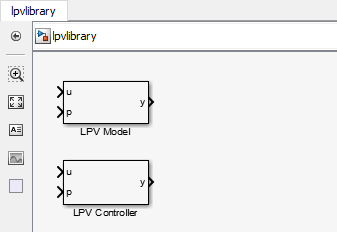
\includegraphics[scale=1]{figs/fig_library.png}
  \caption{\lpvtool simulink library}\label{fig:simulink}
\end{figure}



\bibliographystyle{abbrvnat}
\bibliography{biblio}

\end{document}
